\section{Auswertung}
\label{sec:Auswertung}



\subsection{Überprüfung der Bragg-Bedingung}
\label{subsec:bragg}
Nach der Bragg-Bedingung ist das gemessene Intensitätsmaximum beim Glanzwinkel von $\theta_{theo} = 11,26°$ zu erwarten. \\
Der experimentiell bestimmte Glanzwinkel liegt bei dem verwendeten KBr-Kristall bei $\theta_{exp}=11,25°$ , so wird durch die in \autoref{tab:Tab_bragg} aufgeführten Werte 
der Sollwinkel verifiziert. \\

\begin{table}[H]
  \centering
  \caption{Die Werte für die Messung zur Verifikation der Bragg-Bedingung.}
  \begin{tabular}{cc}
    \toprule
    {$ 2 \cdot \theta \mathbin{/} \unit{\degree}$} &
    {$ N \mathbin{/} Imp / \unit{\second}$} \\
    \midrule
    21,8 &  219,0 \\
    21,9 &  233,0 \\
    22,0 &  249,0 \\
    22,1 &  247,0 \\
    22,2 &  258,0 \\
    22,3 &  259,0 \\
    22,4 &  275,0 \\
    22,5 &  295,0 \\
    22,6 &  289,0 \\
    22,7 &  282,0 \\
    22,8 &  288,0 \\
    22,9 &  287,0 \\
    23,0 &  266,0 \\
    23,1 &  257,0 \\
    23,2 &  266,0 \\
    23,3 &  267,0 \\
    23,4 &  258,0 \\
    23,5 &  244,0 \\


    \bottomrule
  \end{tabular}
  \label{tab:Tab_bragg}
\end{table}




\subsection{Emissionsspektrum}
\label{subsec:emissionsspektrum}


\subsubsection*{Maximale Energie und minimale Wellenlänge}

\begin{figure}
  \centering
  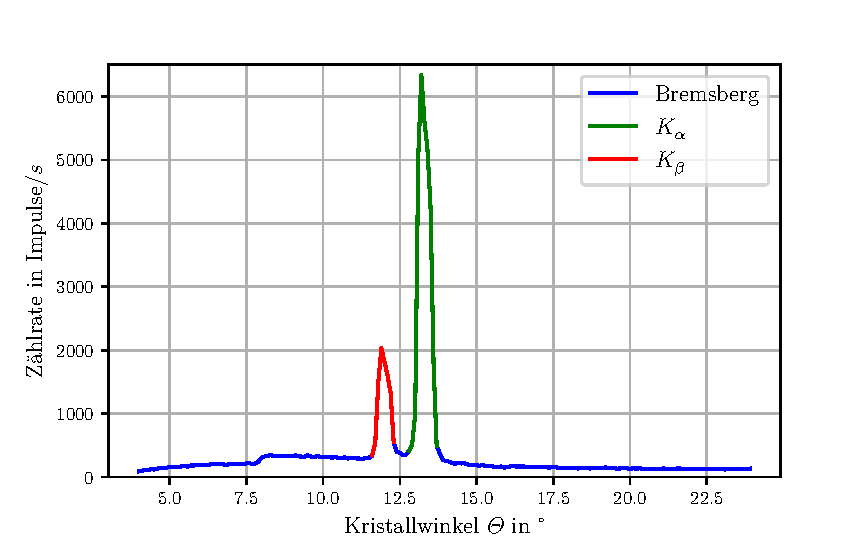
\includegraphics{build/plot_cu.pdf}
  \caption{Emissionsspektrum der Kupfer-Röntgenröhre.}
  \label{fig:cu}
\end{figure}


Das charakteristische Spektrum der Kupfer-Röntgenröhre ist in \autoref{fig:cu} zu sehen.\\
Mit zunehmendem Winkel ist der Grenzwinkel bei  $K_{\alpha}$ und $K_{\beta}$ erkennbar. \\ 
Aus dem Grenzwinkel 
\begin{equation*}
  \theta_{min} = 7,9°
\end{equation*}
lassen sich die maximale Energie und die minimale Wellenlänge 
\begin{equation*}
  E_{max} = 9,137 \mathrm{keV}
\end{equation*}
\begin{equation*}
  \lambda_{min} = 137.5 \si{\pico\m}
\end{equation*} 
berechnen.


\subsubsection*{Auflösungsvermögen der Apparatur}

Mit Hilfe der Halbwertsbreite lässt sich auch das Auflösungsvermögen der Apparatur bestimmen. \\
Die Halbwertsbreite berechnet sich aus den Winkeln $\theta_\beta = 11,9°$ und $\theta_\alpha = 13,2°$.\\
So ergeben sich die Energien zu $E_\alpha = 9,145$ keV und $E_\beta = 8,255$ keV. Aus einem Gaußschen Fit mit Matlab mit der Funktion
\begin{equation*}
  f(x)=a\cdot exp(-((x-b)/c)^2)
\end{equation*} 
ergeben sich mit
\begin{equation*}
  FWHM=2\sqrt{\ln(2)}\cdot c
\end{equation*} 
die Halbwertesbreiten für die jeweiligen K-Linien
\begin{equation*}
  FWHM_{\alpha}=0.4587\ \si{\keV}
\end{equation*}
\begin{equation*}
  FWHM_{\beta}=0.5107\ \si{\keV}
\end{equation*} 
mit denen sich folgende Auflösungsvermögen durch
\begin{equation*}
  A=\frac{E_{\alpha/\beta}}{FWHM_{\alpha/\beta}}
\end{equation*}
berechnet werden können.
Es ergeben sich die Ausflösungsvermögen $\A_\alpha=17.9836$ und $\A_\beta=17.6305$.\\


\subsubsection*{Abschirmkonstanten}

Aus den berechneten Energien $E_{K \alpha}$ und $E_{K \beta}$ und dem Literaturwert $E_{K,\;abs} = 8980.476 \; \mathrm{eV}$ können die 
Abschirmkonstanten $\sigma_1$, $\sigma_2$ und $\sigma_3$ von Kupfer wie folgt bestimmt werden. Die Ordnungszahl lautet $Z = 29$, $n=1$, $m=2$ und $l=3$. \\
Aus 
\begin{equation*}
  \sigma_1=Z-\sqrt{\frac{E_{Kabs}}{R_\infty}}
  \label{eq:sigma}
  \end{equation*}
  
  \begin{equation*}
  \sigma_2=Z-\sqrt{ \frac{m^2}{n^2}(Z-\sigma_1)^2 - \frac{m^2}{R_\infty} E_{K\alpha}}
  \end{equation*}
  
  \begin{equation*}
      \sigma_3=Z-\sqrt{ \frac{l^2}{n^2}(Z-\sigma_1)^2 - \frac{l^2}{R_\infty} E_{K\beta}}
  \end{equation*}
ergeben sie sich zu $\sigma_1 = 3,30$, $\sigma_2 = 13,57$. 
$\sigma_3$ kann nicht korrekt bestimmt werden, da sich ein komplexer Wert ergibt.




\subsection{Absorptionsspektren}
\label{subsec:absorptionsspektrum}


\subsubsection*{Absorptionsspektrum von Zink}
In \autoref{fig:zink} ist das gemessene Absorptionsspektrum von Zink abgebildet.\\
Darin ist die K-Kante bei $\theta = 11,9°$ zu sehen. \\
Nach \autoref{eq:6} ist die ergibt sich die Absorptionsenergie $E_{Zn, \; K} = 9,138 \mathrm{ keV}$.\\
Daraus lässt sich die Abschirmkonstante $\sigma_{Zn, \; K} = 4,08$ errechnen.
\begin{figure}
  \centering
  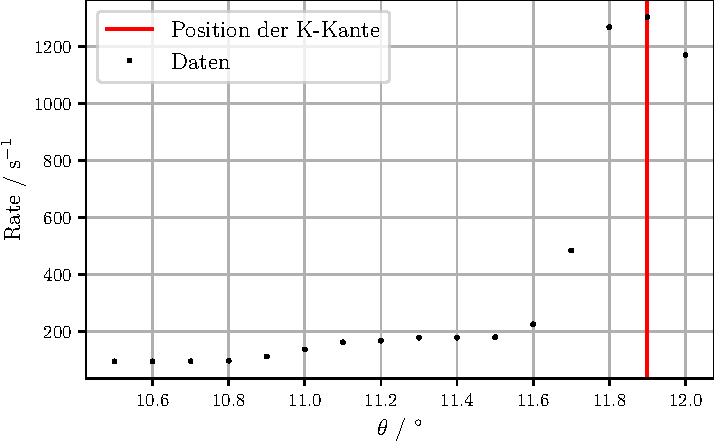
\includegraphics{zink.pdf}
  \caption{Absorptionsspektrum der Röntgenstrahlung von Zink.}
  \label{fig:zink}
\end{figure}


\subsubsection*{Absorptionsspektrum von Gallium}
Im Absorptionsspektrum von Gallium ist die K-Kante bei $\theta = 10,5°$ zu sehen. \\
Nach \autoref{eq:6} ist die ergibt sich die Absorptionsenergie $E_{Ga, \; K} = 10,34 \mathrm{ keV}$.\\
Daraus lässt sich die Abschirmkonstante $\sigma_{Ga, \; K} = 3,43$ errechnen.

\subsubsection*{Absorptionsspektrum von Brom}
Im Absorptionsspektrum von Brom ist die K-Kante bei $\theta = 8,3°$ zu sehen. \\
Nach \autoref{eq:6} ist die ergibt sich die Absorptionsenergie $E_{Br, \; K} = 13,54 \mathrm{ keV}$.\\
Daraus lässt sich die Abschirmkonstante $\sigma_{Br, \; K} = 3,45$ errechnen.

\subsubsection*{Absorptionsspektrum von Strontium}
Im Absorptionsspektrum von Strontium ist die K-Kante bei $\theta = 6,8°$ zu sehen. \\
Nach \autoref{eq:6} ist die ergibt sich die Absorptionsenergie $E_{Sr,\; K} = 15,9  \mathrm{ keV}$.\\
Daraus lässt sich die Abschirmkonstante $\sigma_{Sr, \; K} = 3,81$ errechnen.

\subsubsection*{Absorptionsspektrum von Zirkonium}
Im Absorptionsspektrum von Zirkonium ist die K-Kante bei $\theta = 6,4°$ zu sehen. \\
Nach \autoref{eq:6} ist die ergibt sich die Absorptionsenergie $E_{Zr, \; K} = 16,9  \mathrm{ keV}$.\\
Daraus lässt sich die Abschirmkonstante $\sigma_{Zr, \; K} = 4,75$ errechnen.





\subsubsection*{Moseleysches Gesetz}

Die lineare Ausgleichsrechnung ergibt für die Ausgleichsgerade $y = ax + b$ die Parameter $a = 3,443 \pm 0,2283$ keV und $b = -5,864 \pm 7,9946$ keV.\\
So ergibt sich für die experimentiell bestimmte Rydbergkonstante $R_{exp} = 9,56 \cdot 10^6 \mathrm{\frac{1}{m}}$. 

\begin{figure}
  \centering
  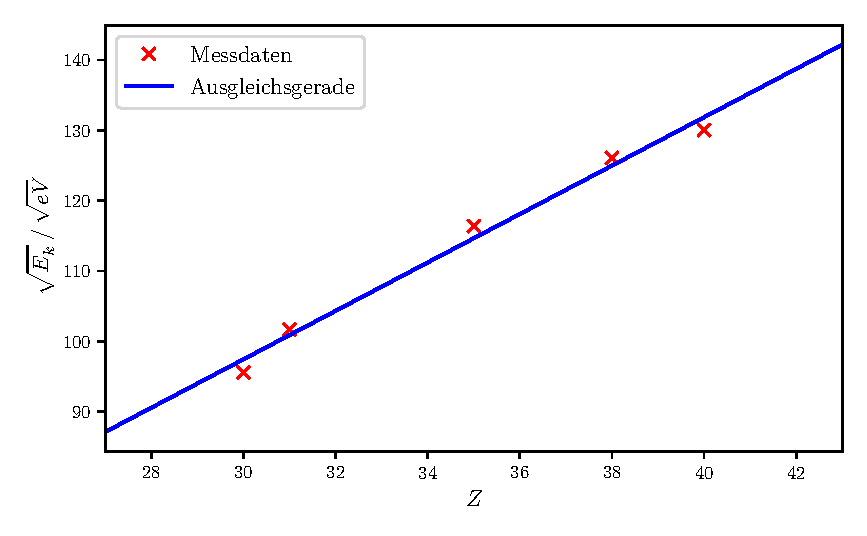
\includegraphics{plot_moseley.pdf}
  \caption{Die Quadratwurzel der Absorptionsenergie in Abhängigkeit von der Ordnungszahl Z mit Ausgleichsgeraden.}
  \label{fig:moseley}
\end{figure}


